% v2-acmsmall-sample.tex, dated March 6 2012
% This is a sample file for ACM small trim journals
%
% Compilation using 'acmsmall.cls' - version 1.3 (March 2012), Aptara Inc.
% (c) 2010 Association for Computing Machinery (ACM)
%
% Questions/Suggestions/Feedback should be addressed to => "acmtexsupport@aptaracorp.com".
% Users can also go through the FAQs available on the journal's submission webpage.
%
% Steps to compile: latex, bibtex, latex latex
%
% For tracking purposes => this is v1.3 - March 2012


\documentclass[prodmode,acmtecs]{acmsmall} % Aptara syntax

\usepackage{amsmath}
% Package to generate and customize Algorithm as per ACM style
\usepackage[ruled]{algorithm2e}
\renewcommand{\algorithmcfname}{ALGORITHM}
\SetAlFnt{\small}
\SetAlCapFnt{\small}
\SetAlCapNameFnt{\small}
\SetAlCapHSkip{0pt}
\IncMargin{-\parindent}

% Metadata Information
\acmVolume{9}
\acmNumber{4}
\acmArticle{39}
\acmYear{2010}
\acmMonth{3}

% Copyright
%\setcopyright{acmcopyright}
%\setcopyright{acmlicensed}
%\setcopyright{rightsretained}
%\setcopyright{usgov}
%\setcopyright{usgovmixed}
%\setcopyright{cagov}
%\setcopyright{cagovmixed}

% DOI
\doi{0000001.0000001}

%ISSN
\issn{1234-56789}

% Document starts
\begin{document}

% Page heads
\markboth{G. Zhou et al.}{A Multifrequency MAC Specially Designed for WSN Applications}

% Title portion
\title{A Parallel Extrapolation Solver for Initial Value Problems in Python}
\author{Humam Alwassel
\affil{Cornell University}
David I. Ketcheson
\affil{King Abdullah University of Science and Technology}
}

\begin{abstract}
Extrapolation methods for ordinary differential equations naturally 
admit an efficient parallel implementation that can take advantage
of typical modern laptops, workstations or compute nodes with several
processors.  We present such a parallel implementation and show that it
outperforms existing standard solvers for a range of problems, as long
as the derivative evaluation is moderately expensive.  The solver is
implemented in pure Python and is thus highly portable and very easy to read.
Features include adaptive step size and order control as well as dense output.
\end{abstract}


%
% The code below should be generated by the tool at
% http://dl.acm.org/ccs.cfm
% Please copy and paste the code instead of the example below. 
%
\begin{CCSXML}
<ccs2012>
 <concept>
  <concept_id>10010520.10010553.10010562</concept_id>
  <concept_desc>Computer systems organization~Embedded systems</concept_desc>
  <concept_significance>500</concept_significance>
 </concept>
 <concept>
  <concept_id>10010520.10010575.10010755</concept_id>
  <concept_desc>Computer systems organization~Redundancy</concept_desc>
  <concept_significance>300</concept_significance>
 </concept>
 <concept>
  <concept_id>10010520.10010553.10010554</concept_id>
  <concept_desc>Computer systems organization~Robotics</concept_desc>
  <concept_significance>100</concept_significance>
 </concept>
 <concept>
  <concept_id>10003033.10003083.10003095</concept_id>
  <concept_desc>Networks~Network reliability</concept_desc>
  <concept_significance>100</concept_significance>
 </concept>
</ccs2012>  
\end{CCSXML}

\ccsdesc[500]{Computer systems organization~Embedded systems}
\ccsdesc[300]{Computer systems organization~Redundancy}
\ccsdesc{Computer systems organization~Robotics}
\ccsdesc[100]{Networks~Network reliability}

%
% End generated code
%

\keywords{extrapolation, initial value problem}

\acmformat{Humam Alwassel and David I. Ketcheson, 2015.  A Parallel
Extrapolation Solver for Initial Value Problems in Python.}
% At a minimum you need to supply the author names, year and a title.
% IMPORTANT:
% Full first names whenever they are known, surname last, followed by a period.
% In the case of two authors, 'and' is placed between them.
% In the case of three or more authors, the serial comma is used, that is, all author names
% except the last one but including the penultimate author's name are followed by a comma,
% and then 'and' is placed before the final author's name.
% If only first and middle initials are known, then each initial
% is followed by a period and they are separated by a space.
% The remaining information (journal title, volume, article number, date, etc.) is 'auto-generated'.

\begin{bottomstuff}
This work is supported by King Abdullah University of Science and Technology.

Author's addresses: 
\end{bottomstuff}

\maketitle


\section{Introduction}
Introduce extrapolation methods here and review previous work.

\section{Parallel Extrapolation}
Describe algorithmic details including parallel load balancing, adaptivity, and dense output.

\section{Numerical results}
In this section we compare our code to $DOPRI5$ and $DOP853$ integrators from $scipy.integrate.ode$. We ran the comparison test on three problems: N-body problem, Burgers' equation, and Korteweg-de Vries (KdV) equation. For each problem, we compared the relative global error in the final solution vs. wall clock time. The reference solutions used for each problem were computed at tight tolerances. The tests were run on a workstation with two 2.66 GHz quad-core Intel Xeon processors.

\subsection{N-body problem}
We tested with $N = 400$. The initial time was 0, and the final time was set to $T = 0.008$.
\begin{figure}[h]
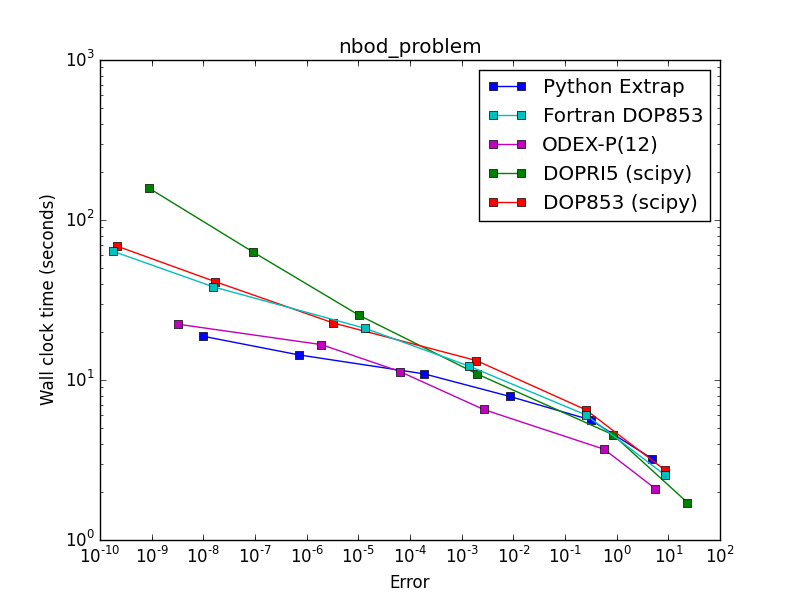
\includegraphics[scale=0.5]{../images/nbod_problem_err_vs_time.png}
\centering
\caption{Runtime versus achieved relative error for N-body problem}
\end{figure} 

\subsection{Burgers' equation ($u_t+uu_x=\epsilon u_{xx}$)}
We transform Burgers' equation to a non-stiff ODE by taking the Fourier transform and replacing each $x$-derivative by $i\xi$. We get the equivalent ODE
\begin{align*}
\hat{U}'(t) = - \frac{i\xi}{2} e^{\left( \xi^2 \epsilon t \right)} 
  \mathcal{F} \left\{
      \left[
          \mathcal{F}^{-1} \left(
              e^{\left( -\xi^2 \epsilon t \right)}\hat{U}
          \right)
      \right]^2
  \right\}
\end{align*}
Here $\mathcal{F}$ is the Fourier transform, and $\hat{U} = e^{\xi^2 \epsilon t} \hat{u}$ ($\hat{u}$ is the Fourier transform of $u$).

We tested with $\epsilon = 0.1$, $x \in [-\pi,\pi]$, and a grid size of $N=64$. The initial time and value were $t_0=0$ and $u(0) = \sin(x)^2$ for $x \in [-\pi,0]$ and $0$ otherwise. The final time was set to $T = 3$.
\begin{figure}[h]
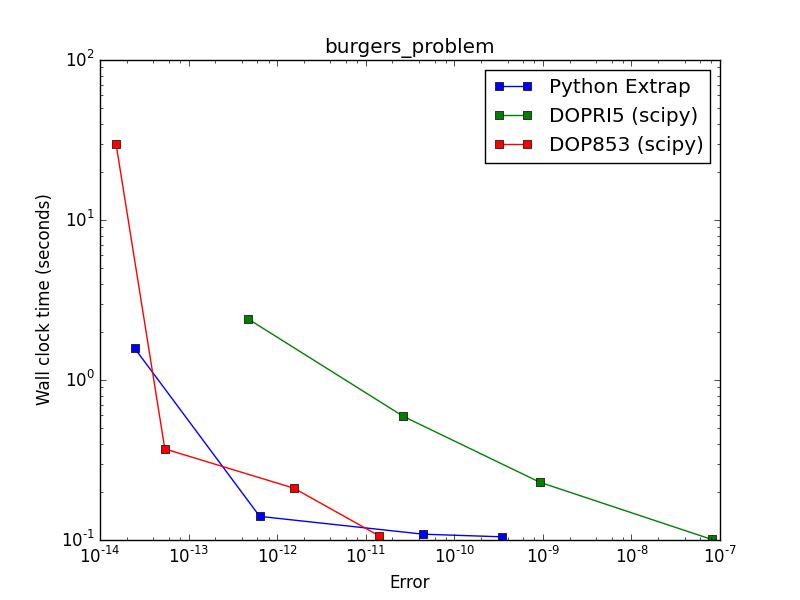
\includegraphics[scale=0.5]{../images/burgers_problem_err_vs_time.png}
\centering
\caption{Runtime versus achieved relative error for Burgers' equation}
\end{figure}

\subsection{KdV equation ($u_t+uu_x+u_{xxx}=0$)}
Similar to Burger's equation, we transform KdV equation to the equivalent non-stiff ODE
\begin{align*}
\hat{U}'(t) = - \frac{i \xi}{2} e^{\left( -i\xi^3 t \right)}
    \mathcal F \left\{
        \left[ \mathcal F^{-1} \left( e^{\left(i\xi^3 t \right)} \hat{U} \right) \right]^2
    \right\}.
\end{align*}
Here $\mathcal{F}$ is the Fourier transform, and $\hat{U} = e^{\left( -i\xi^3 t \right)} \hat{u}$ ($\hat{u}$ is the Fourier transform of $u$).

We tested with $x \in [-\pi,\pi]$, and a grid size of $N=256$. The initial time and value were $t_0=0$ and $u(0) = 3*25^2/\cosh(0.5*(25*(x+2.)))^2 + 3*16^2/\cosh(0.5*(16*(x+1)))^2 $. The final time was set to $T = 0.003$.
\begin{figure}[h]
\includegraphics[scale=0.5]{../images/kdv_problem_err_vs_time.png}
\centering
\caption{Runtime versus achieved relative error for KdV equation}
\end{figure}


% Start of "Sample References" section

\section{Typical references in new ACM Reference Format}
A paginated journal article \cite{Abril07}, an enumerated
journal article \cite{Cohen07}, a reference to an entire issue \cite{JCohen96},
a monograph (whole book) \cite{Kosiur01}, a monograph/whole book in a series (see 2a in spec. document)
\cite{Harel79}, a divisible-book such as an anthology or compilation \cite{Editor00}
followed by the same example, however we only output the series if the volume number is given
\cite{Editor00a} (so Editor00a's series should NOT be present since it has no vol. no.),
a chapter in a divisible book \cite{Spector90}, a chapter in a divisible book
in a series \cite{Douglass98}, a multi-volume work as book \cite{Knuth97},
an article in a proceedings (of a conference, symposium, workshop for example)
(paginated proceedings article) \cite{Andler79}, a proceedings article
with all possible elements \cite{Smith10}, an example of an enumerated
proceedings article \cite{VanGundy07},
an informally published work \cite{Harel78}, a doctoral dissertation \cite{Clarkson85},
a master's thesis: \cite{anisi03}, an online document / world wide web resource \cite{Thornburg01}, \cite{Ablamowicz07},
\cite{Poker06}, a video game (Case 1) \cite{Obama08} and (Case 2) \cite{Novak03}
and \cite{Lee05} and (Case 3) a patent \cite{JoeScientist001},
work accepted for publication \cite{rous08}, 'YYYYb'-test for prolific author
\cite{SaeediMEJ10} and \cite{SaeediJETC10}. Other cites might contain
'duplicate' DOI and URLs (some SIAM articles) \cite{Kirschmer:2010:AEI:1958016.1958018}.
Boris / Barbara Beeton: multi-volume works as books
\cite{MR781536} and \cite{MR781537}.

% Acknowledgments
\begin{acks}
The authors would like to thank...
\end{acks}

% Bibliography
\bibliographystyle{ACM-Reference-Format-Journals}
\bibliography{acmsmall-sample-bibfile}
                             % Sample .bib file with references that match those in
                             % the 'Specifications Document (V1.5)' as well containing
                             % 'legacy' bibs and bibs with 'alternate codings'.
                             % Gerry Murray - March 2012

% History dates
\received{February 2007}{March 2009}{June 2009}

% Electronic Appendix
\elecappendix

\medskip

\section{This is an example of Appendix section head}

Channel-switching time is measured as the time length it takes for
motes to successfully switch from one channel to another. This
parameter impacts the maximum network throughput, because motes
cannot receive or send any packet during this period of time, and it
also affects the efficiency of toggle snooping in MMSN, where motes
need to sense through channels rapidly.

By repeating experiments 100 times, we get the average
channel-switching time of Micaz motes: 24.3 $\mu$s. We then conduct
the same experiments with different Micaz motes, as well as
experiments with the transmitter switching from Channel 11 to other
channels. In both scenarios, the channel-switching time does not have
obvious changes. (In our experiments, all values are in the range of
23.6 $\mu$s to 24.9 $\mu$s.)

\section{Appendix section head}

The primary consumer of energy in WSNs is idle listening. The key to
reduce idle listening is executing low duty-cycle on nodes. Two
primary approaches are considered in controlling duty-cycles in the
MAC layer.

\end{document}
% End of v2-acmsmall-sample.tex (March 2012) - Gerry Murray, ACM


